%----------------------------------------------------------------------------------------
%	PREPROCESSING PIPELINE AND DATASET CREATION
%----------------------------------------------------------------------------------------
\section{The dataset}

Before implementing any approach that allows to predict a label to an asparagus, the recorded image data has to be preprocessed and arranged in a sensible format making it accessible (or even simpler to work with) for any computer algorithm.
It will be described in detail how the raw images were processed into a data set and how we obtained labels for the supervised learning approach. Further, the sorting criteria that were decided on and the evaluation of the label agreement will be summarized. In the end, the classical computer vision approaches that were used to detect certain features from the image data without a machine learning process will be outlined. \\
\\
As a first step, the images were loaded and saved on the university internal store. The images were checked for any general errors and ordered in sets of 10000 images in the single folders on the Grid.
This was followed by different preprocessing steps: the three images of one spear were gathered at one location and the background was removed together with any other unnecessary information in the images. Most of the collected data was not labelled such that a solution to the issue of how to attribute a fitting label to each spear was needed. This proved to be a labour-intensive task for the accumulated amount of data.
The first attempt to classify the unlabelled data consisted of automatically extracting the single features in the image which are responsible for a spear’s label. The idea was to use classical machine learning approaches to obtain the individual features. For example, one can define a threshold for the RGB values in the images to detect colour-based features like rust. As it was not possible to completely extract all features from the pictures (especially the detection of a flower posed great difficulties), it was decided to label the images by hand. For that purpose, first all implementable feature extraction functions were combined in an application to aid the hand-labelling process. \\
The hand-label application has a graphical user interface. With ‘yes’ and ‘no’ buttons, the user clicks through the different feature categories and confirms the presence or absence of a feature. Some of the automatic feature extraction scripts classified an image poorly or even incorrect on their own but could still be used as an assistance to the user of the app. \\
For manually labelling all images with the application, every member of the group had to look through a batch of asparagus images and note whether each feature is present in the image. \\
The manual label process bore its own difficulties as critical images led to indecisiveness in the feature detection and a variance in the overall labelling agreement. The sorting agreement was therefore derived and used as a measurement of the overall quality of the manual sorting process. \\
Finally, the data set was built. To have a unified version of all images and their respective labels, a reading function was created. \\
\\
In this chapter, the different preparatory steps for the recorded data are described, including the creation of a data set which is usable for any machine learning or computer vision approach to analyse the image data. In 3.1 \textit{Preprocessing}, the data is assessed and simplified for any further processing. The second section, 3.2 \textit{Automatic feature extraction}, deals with the creation of feature scripts that were researched and implemented for an automatic recognition of single features.
The results were combined in an application which is described in detail in 3.3 \textit{Manual labelling app}. In 3.4 \textit{Manual labelling}, the process of hand-labelling the images with the application is described, followed by a section analyzing the results and comparing the overall agreement of the labellers. The last section, 3.5 \textit{The asparagus data set}, concludes with the creation of the final data set, used for the later training of the neuronal networks and other approaches to detect the label of a spear from its three images.



\subsection{Preprocessing}

An important and often underestimated step of any machine learning project is preprocessing. After collecting the data, it is not yet in the right format and needs to be altered for the particular purpose that one has in mind. \\
\\
Inside the sorting machine we are working with, the asparagus pieces are transported on a conveyor belt with multiple compartments. Whenever an asparagus piece is in the center, a picture of the three center compartments is taken. That means, each asparagus can be found in three pictures, one in each of the three positions – left, center and right. In our case, the first step of the preprocessing was to combine the three perspectives of each asparagus piece. The image names can be used to combine the three relevant images and determine in which position the asparagus was captured. This way the images can be cut into three pieces and renamed in a way that makes it clear which images belong together. Each asparagus gets a unique identification number and the three perspectives are denoted with “a” for left, “b” for middle, and “c” for right. For example, the image 42\textunderscore b.png is the center image of the asparagus piece with the identification number 42. \\
The second step was to remove the background to trim as much of the unnecessary information as possible. As the conveyor belt is blue, there is a high contrast to the bright asparagus pieces, aiding the background removal. First, the asparagus piece is masked using the hue of the HSV representation of each image. Second, very dark regions are marked as background by thresholding the value component. This is particularly important for the automatic feature extraction (cf. Chapter 4). Additionally, the asparagus was rotated upwards to reduce the variance in angle. The rotation angle is achieved by binarizing the asparagus piece image into foreground and background pixels, calculating the centerline as the mean pixel location along the vertical axis and fitting linear regression to the centerline pixels. The estimates for the angles are retrieved using arcus tangens and the images are rotated accordingly. By doing that, any distortions like reflections or single noisy pixels are set to zero and only the asparagus piece itself remains. The only faulty areas that can be left over with this approach are areas that are connected to the asparagus. The position of the asparagus within each cutted image was further improved by centering the fragments of the image around the center of mass. This way the asparagus is always in the middle. If the new cutting line falls out of the image boundaries, the missing area is filled with zeros. \\
\\
It should be noted that, although it is an advantage to have several perspectives on the asparagus, as some features might only be visible from a certain side, it also bears some problems. Namely, the lighting and reflection are slightly different, which can alter the colour values, and the images can be a little distorted. Hence, the asparagus might appear wider or smaller depending on the perspective. This makes it harder for classical computer vision algorithms to determine some features accurately. \\
\\
Another data set was computed by converting the images to colour palette images. An appropriate palette and the respective mapping of RGB values to palette colours was determined using clustering in colour space. First, a set of RGB tuples is collected by adding pixel values for the depiction of 10.000 asparagus pieces. Second, the resulting list of RGB tuples is converted to an image and third, a palette is determined using a clustering algorithm that determines the position of cluster centers while maximizing the  maximal coverage. The resulting cluster centers can be displayed as a list of RGB values and represent the colour pallette (\url{https://github.com/python-pillow/Pillow/blob/55e5b7de6c41b0386660b0bee7784ac04f412f4b/src/libImaging/Quant.c}, \url{https://www.sciencedirect.com/science/article/pii/S1026309811002100}). Each image of the downscaled data set was transformed to the palette representation. Visual inspection showed little quality loss such that it can be assumed that the relevant information for image classification is well preserved. \\
\\
Several additional data sets were computed based on the data without background. This holds for downscaled versions as well as for a version that contains the asparagus heads only. To compute the latter, the images were padded to avoid sampling outside of the valid image boundaries and the uppermost foreground row was detected. Subsequently the center pixel was determined and the image was cropped such that this uppermost central pixel of the asparagus is the center of the uppermost row of the snippet. The resulting partial images of asparagus heads are rotated using the centerline regression approach described above. The approach has proven reliable and the resulting depictions were used to train a dedicated network for head related features (see 4.1.2).



\subsection{Automatic feature extraction}

Beside the main aim of this study project, to use machine learning algorithms to classify asparagus automatically, also classical computer vision methods were implemented for comparison. We used these methods to write algorithms that take the images as an input and return a prediction for the different features as an output. The goal was to predict the features reliable enough to deduce the corresponding class from them. \\
\\
According to the producer of the used sorting machine, the softwares currently on the market use very similar methods, which gives us reason to believe that the classical methods might not be adequate to yield a better classification than the current status quo. Nonetheless, it is interesting to see, which features are harder to detect and which are easier. \\
The results vary greatly between the different feature extraction methods. While the functions to detect the width and length and whether the asparagus is violet or bended were good enough to be integrated into the hand label app to help us label, other features turned out to be more difficult. \\
\\
In the following, the different automatic feature extraction methods will be described, alongside with the results that were achieved and future steps that could be taken to improve the results further. For each feature detection method, the images with removed background were used.


\subsubsection{Length}

The length detection uses a pixel-based approach, it counts the number of rows from the highest to the lowest pixel that is not a background pixel and therefore not zero. The asparagus was rotated upwards, as described in chapter 3.1, in order to improve the results, as the rows between the highest and the lowest pixel are counted and not the pixels themselves. This technique is a simplification, which does not represent curved asparagus very well, because it will have a shorter count than it would have if the pixels were counted along the asparagus piece. But in reality, there are not a lot of asparagus pieces close to the decision boundary between broken and a whole piece. Usually, the asparagus is picked a few centimeters longer than necessary and then cut to the desired length. The only asparagus shorter than that length are the ones that break while in the sorting machine. And if they break they generally break closer to the center of the asparagus rather than at the ends of it. Therefore, the difference in length detection does not matter for our classification. \\
\\
All in all, the length detection yields good results that are very helpful for the label app. The next step would be to train a decision boundary that determines which number of pixels should be the threshold to differentiate between broken and not broken. At first, we tried to calculate this threshold by finding a conversion factor from pixel to millimeter, as we know the cut off in millimeters. But this approach appeared to be more difficult than anticipated, because the conversion factor varies in the different image positions. This problem only became apparent after the asparagus season had ended, for which reason we could not reproduce the camera calibrations in retrospective in order to take well-measured images, for example from a chessboard pattern. Accordingly, the threshold needs to be deduced from the data or learned with a machine learning approach.

\subsubsection{Width}

The width detection uses a very similar approach as the length detection as it takes the pixel count from the left-most to the right-most  pixel in a certain row as a width measure. But in contrast to the length, the width was measured at several different rows from which the mean width was taken. For the label app we decided that three measurements are sufficient, because asparagus spears usually do not show drastic changes in width at several positions. Hence, if there are larger changes at all, three evenly distributed positions should capture those changes well. \\
\\
The algorithm operates as follows: Firstly, the images are binarized into foreground and background, which means setting all pixels that are not zero, and therefore not background, to one. After that, the upper-most foreground pixel is detected and the length is calculated with the length detection function as described above. The length of the asparagus is used to divide it into even parts. This is done by determining a start pixel and dividing the remaining rows that contain foreground pixels by the number of positions one wants to measure at. This way several rows are selected in which the number of foreground pixels is counted. One can interpret each row as a cross-section of the asparagus, therefore the number of foreground pixels is a direct measure for the width. Then, the mean of these counts is calculated and used as the final width value. As the head of the asparagus can be of varying form and does not represent the width of the whole asparagus well, it is excluded from the measure. This is done by selecting a start pixel below the head area instead of naively choosing the uppermost pixel. To be precise, the start pixel is chosen 200 pixels below the uppermost pixel in order to bypass the head area with certainty. As described in the length detection, also in the case of the width detection curved asparagus pieces might lead to slightly different outcomes than the true values, but again this difference is regarded as irrelevant in our case.

\subsubsection{Rust}

The rust detection finds all pixels that fall in the range of RGB values that correspond to the color brown. Those pixels are counted and normalized by the maximal number of possible pixels that could be rusty, namely the number of foreground pixels. But as it is impossible that the whole asparagus is rusty and hence that all the foreground pixels fall into the relevant range of RGB values, this normalization yields small numbers as results. To give an example, an output value of 0.13 is already considered moderately rusty. The lower and upper bound for the RGB values are set to [50,42,30] and [220,220,55], respectively. That means, all pixels that have a red value between 50 and 220, a green value between 42 and 220 and blue value between 30 and 55 are considered as rust. \\
\\
Visual inspection shows that the rust detection algorithm works well to detect rusty areas and barely misses any rusty parts. But it is difficult to set a threshold for the number of pixels needed to be classified as rusty, because many pixels with a brown color that are distributed over the whole piece are not supposed to be classified as rust. Only clusters of brown pixels are a reliable indicator for rust. To make this intuition more clear, it could be the case that two asparagus have the same number of brown pixels, but in one case they are all connected building a cluster and in the other case they are evenly distributed over the whole asparagus piece. That would mean that, although both yield the same output value, only one of them should be considered as rusty. However, it should be mentioned that this is merely an artificial example to display one draw-back of the implementation. In reality, it is  very unlikely that an asparagus has a large number of brown pixels that are not in fact rust. \\
\\
Nevertheless, it remains unsolved to set a robust threshold that works well on the whole dataset. One problem that cannot be solved algorithmically, is dirt in the sorting machine. If the machine is not cleaned thoroughly and regularly, dirt can be falsely classified as rust as it often falls in the same color range. Another problem can be a change of lighting when taking the images. Both issues can be controlled for easily, but have to be communicated well to the farmers.

\subsubsection{Violet}

Especially when exposed to light asparagus pieces tend to change in colour. An initial shift from the desired white appearance to a slightly rose or violet tone can be observed first. This change in colour, that is considered a flaw according to german quality standards, typically affects the head of asparagus pieces. However in some cases a non-uniform distribution of more or less violet areas can be observed. Moreover, it has shown in practice that colour impression is highly subjective~\citep{luo2000review}. This manifested in discussions of edge cases during labeling. Effects of meta contrast potentially even affect the colour impression on an individual level~\citep{reeves1981metacontrast}. The lack of a formal definition for violet asparagus pieces also poses challenges to approaches of measuring this feature. \\
\\
In a simple approach to measure whether an asparagus piece is violet or not, colour hues are evaluated. More precisely, this strategy is based on evaluating histograms of colour hues that are calculated for foreground pixels of the asparagus images after converting them to the HSV colour space. Pale pixels are removed from the selection by thresholding based on the value component of the HSV representation. Finding the optimal threshold was proven difficult and corresponds to the abovementioned question of what it means for an asparagus spear to be violet. A value of 0.3 was considered a good compromise. All three perspectives were taken into account to compute one histogram per asparagus piece. A score was calculated by summing up the number of pixels that lie within a violet colour range. A second threshold was used as the decision boundary for violet detection. The direct and intuitive feedback in the label app showed the relation between varying thresholds and the prediction. It has shown that lowering thresholds also means the feature extractor becomes more sensitive at the price of a reduced specificity. Best overall matches (accuracies) with the subjective perception were found for very low thresholds. In many cases, however, measurements based on this definition of “violet” did not match the attributed labels. \\
\\
Hence, another sparse descriptor was derived from the input images. However, instead of thresholding pale values and calculating the histograms of colour hues this approach relies directly on the colours that are present in the depiction of an asparagus piece. As the 24 bit representations contain a vast amount of colour information in relation to the number of pixels it is, however, unfeasible to use these as an input. Instead the colour palette images can be used. Histograms of pallete images can serve as the basis to define the feature “violet” in a way that captures more of the initial colour information while being simple and understandable enough to allow for customizations by users of sorting algorithms or machines. As a consensus regarding such an explicit definition is arguably hard to achieve and somewhat arbitrary the descriptor was used to learn implicit definitions of the feature by examples (see XX). \\
\\
It has been shown that explicit ways of directly measuring, in how far an asparagus piece is violet can be implemented but heavily depend on the definition of this feature. As colour perception is highly subjective across and even within subjects~\citep{reeves1981metacontrast}, machine learning approaches that are trained on human labelled data appear to be promising. Using them can help generalizing a definition for the degree to which an asparagus piece is violet.


\subsubsection{Curvature}

Multiple curvature scores can easily be computed based on regression fits to the centerline of an asparagus piece. For example, the parameters of linear or polynomial regression can be interpreted as a description of the curvature of an asparagus spear. However, the question remains if a scalar descriptor that matches with the subjective definition can be derived. \\
\\
Deriving sparse descriptions is based on a two stage approach. In the first stage, the centerline of an asparagus piece is computed because it is considered to be a good description of the curvature of asparagus pieces. Preprocessed images are used as the input where the background is removed and replaced by black pixels. Each asparagus piece is approximately oriented vertically. This means that also for curved pieces the head relies within the top center of the image (see XX). The centerline is computed by binarizing the image into foreground and background and computing the mean of pixel locations along the vertical axis (i.e. for each row). The resulting binary representation shows a single pixel line. It serves as the input to the second stage of curvature estimation. \\
\\
In the second stage, curves are fit to the pixel locations of the centerline. For the simplemost score, linear regression is employed and the sum of squared errors is thresholded and interpreted as a curvature score. This score is small for perfectly straight asparagus pieces and increasingly large for bent ones. As an S-shaped piece is arguably perceived as bent even when the overall deviations from the center line are small a second descriptor was computed as the ratio between the error of a linear fit and polynomial regression of degree three. Thresholding values and employing a voting scheme (e.g. at least one value indicates curvature) for the results for all three perspectives yields a rule to measure curvature. However, it has again proven difficult to set thresholds appropriately to reliably capture the visual impression. Hence, another sparse representation was calculated by fitting linear regression to each of six segments of each depiction of an asparagus piece. A multilayer perceptron (MLP) was trained on the resulting 18 angles per piece (see XX). \\
\\
Calculating a score for curvature is fast and efficient. While the respective approach is suitable to define curvature it does not necessarily meet up with the subjective perception of asparagus curvature. Just like histograms of palette images, curvature scores are the results of feature engineering: The use of extensive domain knowledge to filter relevant features~\citep{zheng2018feature}. They can serve as an input to a machine learning approach that maps this sparse representation to the target categories  (see XX).


\subsubsection{Flower}

The implementation of the flower detection function turned out to be difficult to realize. Several approaches have been tested, but none of them generated sufficiently good results. Two main notions were tried. On the one hand, the shape of the head was used as an indicator for a flower. The idea was that asparagus pieces with a flowery head exhibit a less closed head shape. In other words, the head looks less round and has no smooth outline, but shows fringes. On the other hand, the structure within the head was examined. Supposedly, asparagus with flowery heads exhibit more edges and lines in the head area. In both cases, it was challenging to find a way to discriminate between asparagus with and without flowery heads. One reason for that, is the poor resolution of the camera, that is installed in the sorting machine. With a pixel to millimeter ratio of around one to four, it is even difficult to detect flowers with the human eye. Likewise, the current software in the machine struggles greatly with the classification of this feature as well. There are newer versions of the machine available on the market that have an additional camera which solely takes images of the head of the asparagus piece. This way the inspection of the head improves considerably and the detection of flowery heads should be facilitated (see chapter 2.3).


\subsection{The hand-label app: A GUI for labelling asparagus}

Providing a sufficiently large data set that contains information about target categories is one of the major non-algorithmic challenges in the application of machine learning for classification tasks~\citep{al2018labeling}. In many cases, however, the respective labels are missing. Missing labels are especially problematic if traditional supervised learning methods such as feed forward CNNs are employed: if the variance in the input images is high, a large number of samples is required~\citep{russakovsky2015imagenet}. 
The options to reduce the variance and hence the need for a large labeled dataset are limited. One may rely on preprocessing to reduce the variance. In addition, strategies on the algorithmic domain such as the use of pretrained networks for transfer learning (\url{https://www.learnopencv.com/keras-tutorial-transfer-learning-using-pre-trained-models/}) or semi-supervised learning as well as manual feature engineering by means of traditional computer vision or machine learning (see 4.1.1) may help to retrieve sparse representations without the requirement for training on labelled data sets. As such these approaches promise to reduce the requirement for very large labelled data sets. This does not mean, however, that labelled samples are irrelevant. Without a sufficient number of labelled samples also these approaches fail. In addition, labelled data is essential for the evaluation of machine learning algorithms. Without labels no quality metrics such as accuracies, sensitivity and specificity can be calculated. If target labels are unknown it is hence inevitable to manually generate them. \\
\\
Annotating labels manually is a common practice, however it requires plenty of effort. “Dataset annotation and/or labeling is a difficult, confusing and time consuming task; and even after labeling, it is difficult to assess a dataset for label correctness, whether manually or automatically”~\citep{al2018labeling}. Human performance may be acknowledged as the baseline or “gold standard” that image classifiers are evaluated by (Footnote: For example the performance of GoogLeNet is compared to human level performance using the ImageNet dataset~\citep{russakovsky2015imagenet}). Hence in many scenarios data is labelled by human coders such that machine learning algorithms can be fitted on the training subset of the resulting hand labelled data sets and evaluated on a test subset. This holds especially for image classification tasks~\citep{russakovsky2015imagenet}. In the present case some features were considered to be reliably measurable by means of computer vision (e.g. the width or the length). For features such as a flowering asparagus head or the evaluation whether or not a piece is affected by the rust fungus this has proven to be difficult. Considering the amount of data that could potentially be labelled, a custom interface is required that allows for efficient attribution of labels: For this purpose an app with graphical user interface is developed that allows for efficient attribution of labels. \\
\\
The hand label app comprises two user interfaces. A startup window that allows for a preview of asparagus images and the attributed labels (represented by Ui\textunderscore Asparator) as well as the main labeling interface (Ui\textunderscore LabelDialog). Using the labeling interface is possible only after the user selects the source folder of images and specifies or loads a file that contains the attributed labels. This ensures that the input and output file path are set. A dictionary that maps indices to images can be parsed from filenames and the minimum index is determined. As such the label dialog and the respective controller class always resides in a valid initial state. For labeling, the user answers questions (with yes or no) that are displayed alongside the images that depict each asparagus piece from three perspectives. To facilitate this process the arrow keys can be used. The result is saved and the next question will automatically appear upon answering. \\
In addition, automatic feature detection can be selected for specific features. The result is displayed and saved to a file. The user is not asked to answer questions that target named features and attribute the respective label. This flexible approach was chosen as it was initially unclear and disputed in how far automatic feature extraction yields results that meet up with the individual perception. It also allowed to improve automatic feature extraction methods and to develop a direct intuition for the relation with the data. On top of that it has proven to be useful for debugging automatic feature extraction methods that failed for some images. \\
\\
The development of the app was accompanied by three major challenges. First handling a large data set of several hundred gigabytes that is accessible in a network drive. Second, changing requirements that resulted from group decision processes with respect to automatic feature extraction as well as from unforeseen necessities in (parallel) preprocessing and made substantial changes of the initial architecture and the reimplementation of parts of the code necessary. The third challenge was the related question of the handling of internal states of the app. The latter may be further explained. \\
\\
Internal states of the app were handled such that it is possible for the user to navigate into invalid states for which no images are available. The reason for this choice may be explained shortly. Note that preprocessing was done such that each asparagus piece has a unique Integer-ID and a specifier for perspectives a, b and c in it’s filename. While generally IDs are in a continuous range from zero to n some indices are missing. As preprocessing jobs were scheduled to run in parallel and preprocessing failed for few corrupted files it has proven almost inevitable to end up with few missing indices although a dictionary of input filename and output filename was passed to each grid job. In addition, the large amount of data did not allow to save all files in a single directory. In summary this means that one could not simply iterate over asparagus IDs (represented by the state of a spin box in the user interface), determine the file path and display the related images. Instead parsing filenames from a slow network drive is necessary which requires limiting the number of selected pieces. As GUI elements such as spin boxes and keyboard controls allow for setting an integer, and it was a requirement that this integer relates to the asparagus ID, one ends up with the following situation. Either one prevents that the asparagus ID is set or incremented freely to a value that does not exist or one allows to navigate into an invalid state. It was decided that it is the most simple approach to allow the app to have an inconsistent state where the current ID is invalid because there is no respective data (Footnote: The earlier approach showed to have several implementation specific drawbacks. Note for example that upon entering multiple digits in an input field an event is triggered multiple times. Upon entering the value 10 for the asparaus ID one ends up with the value being set to 1 before being set to 10 where 1 relates to a potentially missing ID. This means the user could not freely enter IDs when setting them to specific values is impossible.). Hence, all cascades of methods of the app including preprocessing functions that require the respective images as an input were adjusted such that they can handle this case. \\

\begin{figure}[h]
	\centering
	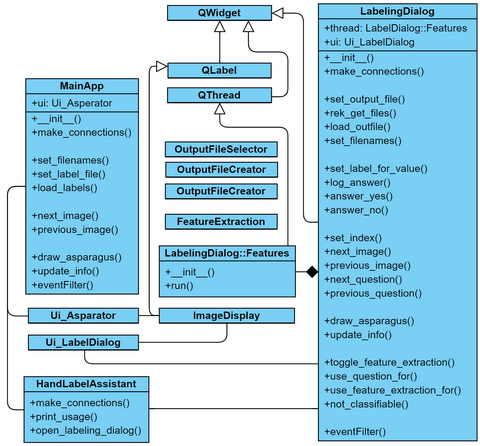
\includegraphics[scale=0.6]{Figures/chapter03/label_app_tree}
	\decoRule
	\caption[??]{??}
	\label{fig:LabelAppTree}
\end{figure}

The app is implemented using the PyQt5 framework while coarsely following the model, view controller principle. No separate database and the respective model class is used. The data model is implicitly parsed from the filenames and administered in attributes of the view. The labels are administered as a Pandas DataFrame and serialized as a csv-file. Upon state change (i.e. index increment) images are loaded from the network drive that was mounted on the level of the operating system. The views are designed using QtDesigner. Four manually coded classes are essential for the architecture of the app: The class HandLabelAssistant in which the PyQt5 App is instantiated, the controllers MainApp and LabelingDialog as well as Features which is member class of the latter, of type QThread and represents the API to the automatic feature extraction methods in FeatureExtraction. Ui\textunderscore Asparator, UiLabelDialog and classes for file dialogs represent the views. A class ImageDisplay is required to display images with the correct aspect ratio. The figure below shows the UML class diagram alongside methods and attributes that are considered relevant to understand the architecture of the app. \\
Developing a custom app for the labeling process required substantial time resources. However, it was found that existing solutions did not meet the specific requirements. Our custom hand label app allowed us to attribute labels for more than 10.000 labels in a manageable amount of time. Details of the labeling process are described in the next section.

\subsection{Manual labelling}

In this section of chapter 3, the process of manually labelling the data with the help of the hand-labelling app is laid out. It includes the sorting criteria which allocate each spear to a single asparagus class, the practice of manually labelling the preprocessed data for its features, the outcome of the labelling process, and the approach to measure the agreement of the manual labelling are described in more detail. \\
\\
The images were classified by all members of the group. As none of the group participants are experts of labelling asparagus, a general guideline for the labelling had to be established which is elaborated in detail in the following subsections. The guideline is written in accordance with the owner of the asparagus farm of “Gut Holsterfeld”, Mr. Silvan Schulze-Weddige. He was consulted in all questions regarding the sorting of the asparagus. \\
General challenges in the manual sorting in front of a computer screen, including the respective image quality, and especially the variance in the agreement of the project members were expected from the start. As the task relies on the subjective view of single humans, opinions about the affiliation to one asparagus class can diverge in critical or vague cases.  This is demonstrated in that the seasonal workers who usually sort the asparagus by hand do not agree on every case. Further, a classification session with Mr. Schulze-Weddige was held in which the project members learned to distinguish the different features that decide the class of an asparagus spear. During the session, again it emerged that some images containing critical spears - that is, where the features are not apparent - were hard to classify even by the expert. \\
To tackle the issue and to have an overview of the general agreement of the sorting between group members of the project, a measurement unit was researched and applied, namely the Kappa Agreement. It was applied on a smaller subset of pre-sorted asparagus pieces in the beginning of the manual labelling and a second time at the end of the manual sorting process. The Kappa Agreement was used to assess the degree of accordance in sorting between the single members and monitor how the sorting agreement developed during the manual labelling process. \\
\\
The first subsection, 3.4.1 \textit{Sorting criteria}, expands on the guideline used for categorizing each spear of asparagus according to its features (into a single class).
In the second subsection, 3.4.2 \textit{Sorting outcome}, the process of the manual sorting is shortly described and the achieved results are presented.
The ensuing third subsection, 3.4.3 \textit{Agreement Measures}, and fourth subsection, 3.4.4 \textit{Reliability}, focuses on the Kappa Agreement, which we chose as an evaluation measurement for the accord of our sorting, and the results of applying it are discussed.


\subsubsection{Sorting criteria}

The class of an asparagus spear is decided by several factors, ranging from its shape to its colour. Put together, these single features give us the label for the spear. As it was decided to label the images for their features, the features were checked by the labellers. The images were displayed with the hand-labelling app and the features are divided as follows: ‘fractured’, ‘hollow’, ‘flower’, ‘rusty body’, ‘rusty head’, ‘bent’, ‘violet’, ‘very thick’, ‘medium thick’, ‘thick’, ‘thin’, ‘very thin’. Further, images that could not be sorted thoroughly were sorted as ‘not classifiable’ (e.g. when the spear is cut off the image). \\
To some extent, the manual feature categorization was influenced by the price that each category of asparagus earns. High quality pieces (i.e. 1A Anna) should be thoroughly examined and sorted more conservatively. \\
In the following text, the different criteria for manually labelling the data images for their corresponding features are described. \\
 \\
\textbf{Fractured} \\
An asparagus spear includes the feature ‘fractured’ when it is broken, or if it does in any other way not fulfill the required length of 210 mm.
First, the feature was labelled manually but the procedure was abandoned shortly after because it can be derived  more precisely from the computer-vision based feature extraction ‘length’, which is automatically calculated within the labelling app.
It is then discerned between a fractured piece with a head and a fractured piece without a head. Whenever a spear was fractured but with the head part still attached, it was sorted like a usual, intact asparagus. However, if the head part of the spear was damaged or missing completely, no other features were chosen but the asparagus was labelled as ‘not classifiable’. \\
 \\
\textbf{Hollow} \\
The feature ‘hollow’ indicates that the spear is hollow inside.
This might be expressed by a bulgy center and a line running vertically along the spear’s body. Another, more distinct indicator is when the piece looks like two spears fused together, forming a single asparagus. A hollow asparagus can be confused with a very thick asparagus. \\
The feature can be easily checked when you have physical access to the asparagus. If the asparagus is actually hollow, it will have a hole at its bottom which you can see when turning the spear around. Unfortunately, this cannot be done when only looking at images from the side. The feature hollow sometimes even occurs without showing a clear line or obvious bulge at its center. Therefore, there is a risk of wrong classification. \\
 \\
\textbf{Flower} \\
The asparagus piece is sorted as ‘flower’ when the head part forms a recognizable flower.
For a blooming asparagus, a jagged pattern (slightly resembling a crown) can be seen at its head region. Also, the tip of the head part can be an indicator if it resembles a pointed cap and the petals are visible. When a spear is in full bloom, it is clearly observable. However, the distinction between a spear with clear-cut but closed petals and a spear which just started to develop a flower can be quite difficult. \\
The feature was sorted less strict in uncertain cases where the flower is not clearly distinguishable. One argument is that the flower does not develop further after the sorting process (e.g., as it happens with the feature ‘violet’). Another reason for a less conservative approach regarding the feature ‘flower’ was to lessen any agreement errors in between the manual sorters. It was decided to sort a spear without a rather clear flower as not having the feature ‘flower’. \\
 \\
\textbf{Rusty body} \\
If a spear has rust on its body, it is visible as a dark brown colour.
It often starts at the tips of the leaves or at the bottom part. In severe cases it spreads over the whole asparagus piece. The colour is not light brown but of a dark shade. The colour is not to be confused with bruises, pressure marks, or a slightly yellow complexion (which can occur in a mature asparagus) which are of no further concern to us.
The feature was sorted more strictly to facilitate the decision process during the manual sorting. Therefore, ‘rust’ was set to be present even when only the tip of a leaf showed a dark spot. Other brownish bruises were not classified as rust. \\
We decided to split the feature ‘rust’ into the sub-features ‘rusty body’ and ‘rusty head’. In the case of rust being only on the body, it might still be removable by peeling. If there is rust on, or very close to the head, however, it is not removable. \\
 \\
\textbf{Rusty head} \\
If there is a dark spot on or close to the head region recognizable as rust, it is captured by this feature. The head part is usually distinct in shape and colour from the body part of the asparagus. \\
In principle, the same guidelines applying to ‘rusty body’ can be transferred here, with an explicit focus on the top part (until around 1 cm below the collar) of the asparagus. Rust at the head can be confused with shadow caused by the petals and the luminance  of the sorting machine. Also, it might be that the head is actually violet and not rusty.
As rust at the top part of the spear cannot be removed without damaging the head, it is more decisive for the later categorization into a price class, if the head has rust. \\
 \\
\textbf{Bent} \\
A piece is categorized as bent, if the shape of the asparagus is curved and not straight.
Further, a spear counts as bent whenever it changes the growing direction - that is, it resembles an S curve. If it is only slightly round but can otherwise be thought of as straight and fitting next to other straight pieces without standing out, it is sorted as not being bent. If the spear looks close to the same on all three pictures, it might indicate that it is heavily bent and therefore cannot be turned on the machine’s conveyor belt. \\
Like the feature ‘flower’, though, the feature bent has a broader range of shapes where the piece is not obviously deformed but also not completely straight. In an indecisive case, it was sorted less conservative. exception holds for S-shaped pieces, which always count as bent.\\
 \\
\textbf{Violet} \\
The feature ‘violet ‘indicates whether an asparagus piece is of violet colour.
The shift of colour from white to violet occurs most often around the head region - either at the tip of the head or just below the collar of the head region. However, the piece can also be violet on the whole body. \\
Here, it is crucial to sort thoroughly because the spear will darken further after the sorting. Thus, even a slightly pink spear was sorted as being violet.
 \\
 \\
\textbf{Thickness and length} \\
The thickness and the length were features we did not consider recognizable by view alone (except for extreme cases). Therefore, both features were measured automatically with scripts written and implemented into the manual sorting app. The division into different categories of thickness can be inferred by the overall thickness of the spear.\\
 \\
\textbf{Not classifiable} \\
Whenever an image was damaged, the spear was unrecognizable, the head part of the spear was severed, two separate spears were present on one picture, the spear was cut off by the image, or other unusual circumstances on the image occured, it fell into the category of not being classifiable. The image was not further checked for its features, i.e. as bent, violet, etc., but only marked as being not classifiable.



\subsubsection{Sorting outcome}

In this section, the process and the results of the manual sorting are presented.
During the overall sorting period no major problems occurred that led to any breaks or even the abortion of the labelling process. \\
\\
Whenever an image was manually sorted in our hand-label application, the chosen labels were saved in a csv-file. As csv files are plain text files, all stored values are strings arranged in a table. The first line of the table serves as the heading, attributing each entry in the first column to a feature. As seen in the figure~\ref{fig:CSVfileOverview}, the features are noted in the first column, with the first entry being the image ID. Every feature is separated by a semicolon and can be of value 0.0, 1.0, or empty. Hence, whenever a feature was present in an image, the value was set to 1.0, while, if the feature was not present, it was set to 0.0. For the “not classifiable” labelled images, no value was given to any other feature. In such cases, all other manually selectable labels are left empty. The image path to every of the three images (a, b, and c) for one spear was also saved in the label file in a separate column. After the labelling process, the single csv-files with the labels were merged into one large combined\textunderscore new.csv file which was later used for the classification of the data with the different computer-vision approaches. It can be found in the study project’s Github repository under XX. \\
\\
\begin{figure}[h]
	\centering
	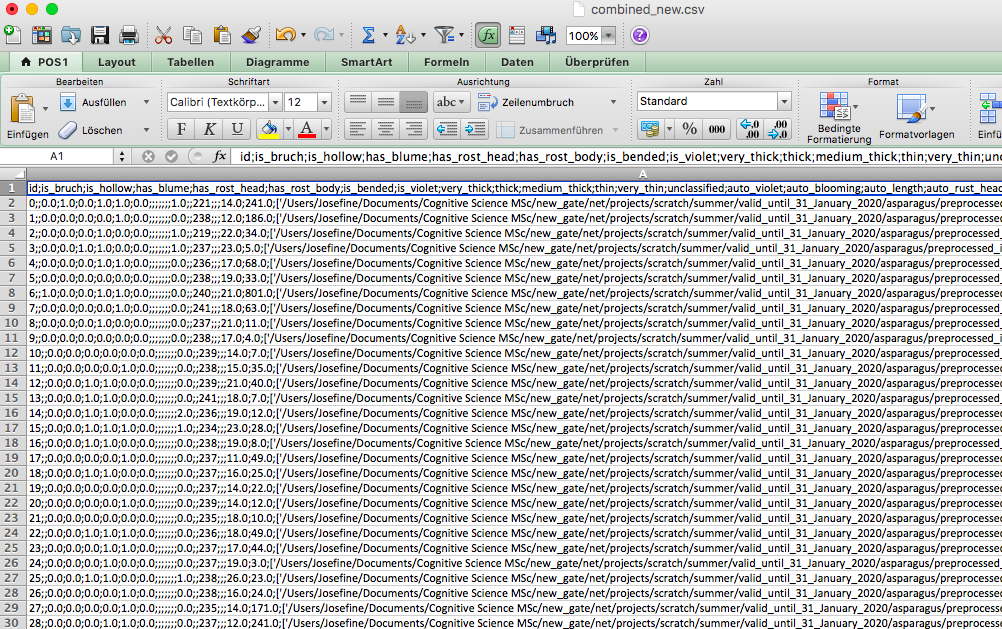
\includegraphics[scale=0.4]{Figures/chapter03/csv_overview}
	\decoRule
	\caption[Manual labelling output csv-file]{The feature labels extracted by the manual sorting process were saved in a csv file. This image shows the beginning of combined\textunderscore new.csv in which all label files were later combined to one file.}
	\label{fig:CSVfileOverview}
\end{figure}
\\
The manual sorting lasted over the period of November 2019 to January 2020.
A session usually consisted of 500 images, with an asparagus spear being viewed in three positions from the same perspective. A session of sorting 500 images took around two to four hours. One minor factor sometimes influencing the time spent for sorting were difficulties with the external connection to the IKW store, as all images are stored on the university servers and it was sometimes worked from home. Another factor was the large number of pictures, with some spears obviously incorporating certain features, while others needed more careful examination. The average time spent for sorting one spear (i.e. noting all features present) was around 27 - 48 seconds. \\
All in all, 13319 triples of images were labelled for their features.
There is a large variance in the presence of the features in the data. Some features were occurring more often than others. Of the acquired 13319 images, the individual features are represented as follows: 3.5\% fractured asparagus pieces, 3.3\% hollow, 12.9\% flower, 14.7\% rusty head, 45.5\% rusty body, 40\% bent, 7.9\% violet, and 2.1\% not classifiable images. Further categories that were not manually assessed but calculated from the automatic thickness detection included 4\% very thick (i.e., above 26 mm), 29.1\% thick (20 - 26 mm), 18,7\% medium (18 - 20 mm), 17.9\% thin (16 - 18 mm), 30.3\% very thin (below 16 mm). A further feature calculated automatically was the length of each spear. All images that were not classifiable are excluded from the calculation of the thickness in the stated numbers. \\
As can be seen, many features are only sparsely present in the data. This poses an imbalance that is relevant for later classification tasks and the usage of the data set.
Further, every member of the group participated in the sorting but not everybody sorted the same number of images. Due to this circumstance, the sorting bias of certain members is more present in the data than of others. \\
The manual sorting was stopped when the amount of classified data exceeded 13000 samples. That is, the less present features (hollow, violet, and flower) were in advance assumed to have a presence of around 8\%. In order to have at least 1000 images with such a feature present, a threshold of 13000 labelled samples was set in advance. The manual sorting was put to a halt when this threshold was reached. \\
\\
As different people were sorting the asparagus and because the decision boundary for sorting a spear is flexible/subjective to the human eye, a measurement was needed that explores how well the members agreed in the labelling process. Thus, at the beginning and at the end of the manual labelling, images were taken and scrutinized for their features. This was done to train the labellers but also to have a test set for the agreement measure. Every category was therefore sorted by at least two labellers separately and their agreement was compared. More details about the method that was chosen to assess the group’s sorting accuracy can be found in the following section 3.4.4. \textit{Reliability}.


\subsubsection{Agreement Measures}

When different annotators label data, it is indispensable to verify the degree of agreement among raters. In order to judge how consistently the data is labeled, several statistical methods (inter-rater-reliability) can be applied. \\
 \\
For the current purpose, different agreement measures, all implemented by scikit learn, were used. The first was Cohen’s Kappa. It was chosen, as it is seen as a more robust measure than a simple agreement percentage, such as a measure of true positive and true negatives, which was traditionally used for those cases~\citep{cohen1960coefficient}. It is more robust, as the rate of agreement occurring by chance is included in the calculation. This method is applicable to compare the rating of two raters on a classification problem. This measure of agreement always lies between -1.0 and 1.0, inclusively. The higher the Kappa value, the higher the agreement. Values around 0 indicate no agreement and negative values indicate negative agreement, so to say systematic disagreement. Values between 0.41-0.6 are seen as moderate agreement, 0.61-0.8 as substantial agreement, and everything above as almost perfect agreement. Everything below 0.4 is interpreted as not acceptable (\url{https://www.ncbi.nlm.nih.gov/pmc/articles/PMC3900052/}). \\
\\
Another statistical method used to measure agreement is the F1 score. The F1 Score is used for the evaluation of binary classification. The F1 score relies both on the precision, as well as the recall of a test’s accuracy. A F1 score value lies between 0 and 1, the higher the F1 score, the higher the agreement. \\
\\
Lastly, we looked at the accuracy measure. For a normalized accuracy score, the values lie between 0 and 1, and the best performance is 1. This measure returns the fraction of correctly classified samples. It is a less robust measure than Cohen’s Kappa score.

\subsubsection{Reliability}

In order to evaluate the degree of agreement of our data, we made agreement measures at two points in time (Footnote: for our API documentation see: \url{https://asparagus.readthedocs.io/en/latest/api/measure\textunderscore agreement.html}). The first time, six different annotators labelled images out of each asparagus group (13 class labels). We ensured that always two different annotators labelled the same set of images. Results were not as good as hoped for. The Kappa scores varied strongly between groups and features from -0.03 to 0.76, while the accuracy scores ranged from 0.49 to 1. It seemed untypical to us, that the agreement scores were so low, even though the raters give the same label to many of the asparagus pieces. This is a known problem~\citep{powers2012problem} ~\citep{sim2005kappa} ~\citep{feinstein1990high}(\url{https://www.sheffield.ac.uk/polopoly\textunderscore fs/1.404095!/file/RSS\textunderscore Poster\textunderscore Laura\textunderscore Flight\textunderscore Final.pdf}). \\
\\
\begin{figure}[h]
	\centering
	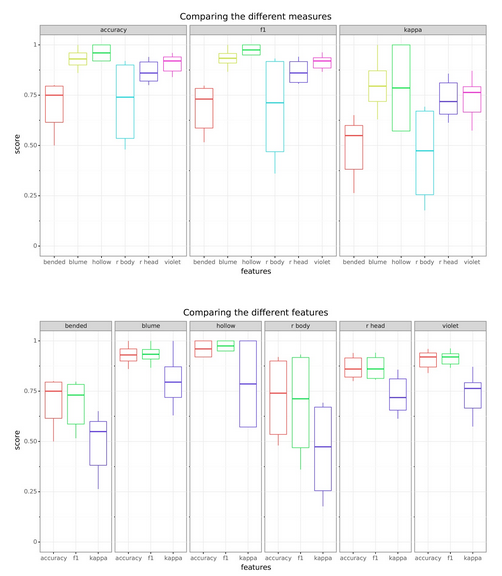
\includegraphics[scale=0.6]{Figures/chapter03/kappacompare}
	\decoRule
	\caption[Agreement measures]{The upper figure shows the agreement measures accuracy, F1 and Cohen’s Kappa, separately for each manually labelled feature. Shown are the box-plots, so the middle line indicates the median, the box indicates the IQR. All scores are aggregated scores over all annotator pairs. The lower figure shows each feature separately. For each feature, the corresponding accuracy, F1 and Cohen’s Kappa score is given. Shown are the box-plots, so the middle line indicates the median, the box indicates the IQR. All scores are aggregated scores over all annotator pairs.}
	\label{fig:KappaCompare}
\end{figure}

One reason for our results could be that we compared the agreement group-wise. This means that we already knew in advance that for certain features, we have almost only 1s or almost only 0s for all images of one group. For Kappa scores, if the distribution of 0s and 1s is not balanced, disagreement of the underrepresented value is punished more heavily (Footnote: see also: \url{https://stats.stackexchange.com/questions/47973/strange-values-of-cohens-kappa}). Therefore, we decided to repeat our agreement measure and do it this time feature-wise on non-labeled images, so that the annotators could not anticipate a specific group label. In order to better understand the reliability of our data, we also decided to look at the accuracy score and the F1 score, additionally. Before we did so, we labeled another 50 images all together, clarified classification boundaries again and discussed unclear images. \\
\\
The second time, 50 images were labeled by 4 annotators. The agreements were measured annotator-pair-wise, and then averaged. The results in the Cohen’s Kappa score vary between and within features, and also between annotator pairs. However, the results are much better than the first time. The highest aggregated kappa score over all annotator pairs is reached for the feature flower (0.79), then hollow (0.79), violet (0.76), rusty head (0.72), bent (0.55) and lastly for rusty body (0.47).
For the features flower, rusty head and violet, the interquartile range (IQR) is quite small, whereas the IQR for hollow, bent and rusty body is much larger (see Figure~\ref{fig:KappaCompare} and XX - both figures).  \\
\\
The agreement scores accuracy and F1 yielded very similar results. Results were slightly better than the Kappa scores, in total and  for each feature. The highest accuracy score is reached for the feature hollow (0.96), then flower (0.93), then violet (0.92), then rusty head (0.86), then bent (0.75) and then rusty body (0.74). The order is the same for the F1 scores. The median F1 scores lie between (0.71 and 0.97). \\
\\
All in all, one can therefore say that the agreement scores indicate moderate up to substantial agreement. Agreement is highest for the features flower, violet and rusty head.


\subsection{The asparagus dataset}

It was described how the data was collected and stored on the IKW storage. After saving, the images were pre-processed and saved in a selected structure. Additionally a CSV file with labels for classifications was created. In this subchapter it is described how the images were processed to be able to use them with models in the future.After giving a theoretical overview of the different possibilities, an assessment follows of what our ideal would have been in the project best practice.  In addition, a description is given which of the existing methods we have used in practice. These methods are compared and followed by a recommendation for further work with the data set. \\
One question arising in regards to modeling a dataset was: what is the best way to provide a model with the image input and corresponding information? There is more than one answer to this question, which makes it more difficult than initially expected. Building the input pipeline in a machine learning project is always long and painful and can take as much time as building the models themselves. First, it is described which common methods are used to prepare the data. We introduce the methods of simply using raw data, saving a NumpayArrays/Tenors or a TFRecord file and the tf.data API and the tf.data.data set API. 
The most straigth-forward variant is to build the model first, then read in the data ,and load the samples one after the other. APIs such as OpenCV, or Imeagio help with this. Here,the possibilities of Python are an advantage. By far the shortest time needed to implement is to load the images from the network memory, our folder structure, and then make them available to the network. However, the runtime is slow, and further processes (described below) are not efficient. Additionally, there may be an overflow and large amounts of data do not fit into the memory. 


\begin{figure}[h]
	\centering
	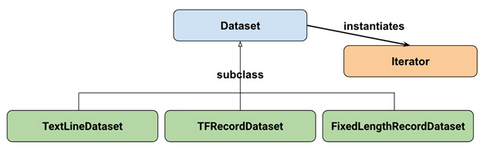
\includegraphics[scale=0.6]{Figures/chapter03/dataset_tf}
	\decoRule
	\caption[??]{??}
	\label{fig:DatasetTF}
\end{figure}

\begin{figure}[h]
	\centering
	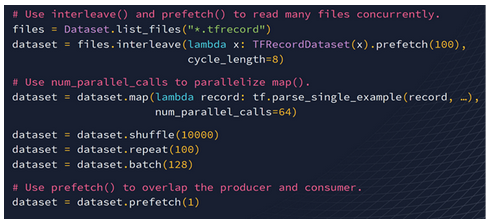
\includegraphics[scale=0.6]{Figures/chapter03/dataset_code}
	\decoRule
	\caption[??]{??}
	\label{fig:DatasetCode}
\end{figure}

Speichern eines Numpy Arrays/Tensors: SOPHIA \\
Additionally, we created a single numpy data set for the labelled images that could be easily stored and loaded for training. Firstly, all the identification numbers from the label files were selected and the corresponding images were found and copied to a separate folder. This folder contains all the images for which we have labels. Secondly, the images were grouped by their identification number, which means the three perspectives of each asparagus spear were combined. We decided to downsample the images for creating this data set to facilitate the training process and reduce memory consumption. Initially, each image was downsampled by a factor of six, that means every 6th pixel was used in the reduced image, but this factor can be easily changed and a new data set will be created for the individual needs of each approach. After that, they were transformed to a numpy array and concatenated to a single file. The images were either concatenated horizontally, so that in the resulting image the three perspectives appear to lay next to each other, or vertically, so that the images are stacked one after another. Finally, all the concatenated arrays were combined to a single four dimensional data set. The first dimension depicts the number of labelled asparagus spears, the second and third dimension represent the height and the width of the images, respectively.  Further, the fourth dimension represents the depth, which is three for the horizontally concatenated images, namely the RGB values, and nine for the vertically stacked images. \\
\\
In the following, Tensorflow's own binary storage format TFRecord is introduced. This approach facilitates the mix and match of data sets and network architectures. Especially because we have huge amounts of data XXXXXX TB, it will have a significant impact on our import pipeline and, therefore, on the total training time. The file format is optimized for images and text data sets. These are stored in tuples which always consist of file and label. The binary files from 100MB to 200MB in size not only take up less space in memory, but can also be read more efficiently. This makes even more difference in our case because the data is stored in the network and not on an SSD hard disk on the PC. The serialized file format allows the data to be streamed efficiently through the network. Another advantage is that the file is transportable over several systems, regardless of the model you want to train with it. \\
\\
Working with TFRecord also simplifies the next steps of .... For example, the division into train set, test set and validation set in a folder structure is no longer necessary and also the mixing of data is no longer needed. These functions are possible with the data format dynamically in any position.  \\
\\
how to build a TFRecord? (In brief) \\
Any data in TFRecord has to be stored as either a list of bytes, a list of float, or a list of int64 only. Each of these created data list entities has to be wrapped by a Feature class. Next, each of the features is stored in a key value pair with the key corresponding to the title being allocated to each feature. These titles are going to be used later when extracting the data from TFRecord. The dictionary created is passed as input to Features class. Lastly, the features object is passed as input to Example class. Then this example class object is appended into the TFRecord. \\
\\
After the TFRecord files were built, it was time to read the data efficiently and create the dataset. With Tensorflow release, 1.4 tf.data was introduced. With the tf.data API it became possible to create complex input pipelines from simple, reusable parts.\\
\\
Tf.data even makes it possible to edit large data sets. The preferred pipeline for our asparagus project is to apply complex transformations to the images and combine them into stacks for training, testing and validating in arbitrary ratios. \\
\\
These "like lazy lists" are not really a new idea. The principle can be found in most mainstream languages like C#'s LINQ or Java 8's streams.  \\
\\
Tf.data provides two interfaces. Firstly, a dataset can be created from a source in several ways. Secondly, a dataset can be changed, e.g. by using different labels or just by transformations like mapping, repeating, batching, or many others. These dozens of transformations can be combined, where a classical order is described in the following. \\
\\
Order of the operations \\
To summarize, one good order for the different transformations is:
\begin{enumerate}
\item create the dataset
\item shuffle (with a big enough buffer size) 3, repeat
\item map with the actual work (preprocessing, augmentation…) using multiple parallel calls
\item batch
\item prefetch
\end{enumerate}
\\

Besides the described functional transformations of the input pipeline under tf.data.dataset, there is an iterator which gives sequential access to the elements in the dataset. The iterator stays at the current position and gives you the possibility to call the next element as a tuple of testors. With initializable iterators, you have the possibility to run through the dataset several times. In addition, you can pass different parameters to start the call. This is especially handy when searching for parameters. \\
\\
In summary there are two advantages. On the one hand, there is the possibility to build a dataset with different data sources. On the other hand, there are many functional transformations and an illerator with sequential access to the data. \\
\\
Derek Murray recapitulates: “If you compare a tf.data pipeline to the equivalent queue-based pipeline, we use a similar structure of queues and threads, but importantly there are no Python queue runner threads on the critical path, and so the tf.data pipeline isn’t constrained by the Global Interpreter Lock and it scales to much higher throughputs.” \\ (\url{https://docs.google.com/presentation/d/16kHNtQslt-yuJ3w8GIx-eEH6t\textunderscore AvFeQOchqGRFpAD7U/edit#slide=id.g254d08e080\textunderscore 0\textunderscore 10}) \\
\\
At the beginning of the development of the dataset, there was the misunderstanding that one of the possibilities was to create a single object which represents the dataset. The most promising one seemed to add directly to the TFDS. \\
\url{https://www.tensorflow.org/datasets/beam_datasets} \\
\\
This would enable the user to get the dataset directly from tensorflow api. For this, we would have needed to publish the data, which would have been no problem. The documentation was not that far advanced at that time, so we spent a lot of time on it. Especially the large amount of data was a problem. Questions like: "How do we deal with the fact that only a part is labelled" or "How should we enter the labels: each as a feature, in a list, or as several features?”. It would have been faster and more helpful for the development of the networks if we had continued to search and integrated the TFRecord files with the tf.data api in our pipeline. So we needed a lot of time and effort that was ultimately lost. 
